\chapter{Path Optimization for Humanoid Walk Planning: an Efficient Approach}
\label{chap:path-optim}

The problem of humanoid motion planning can be defined as the
following: given a starting configuration -- say a position -- we
would like an anthropomorphic system -- say a humanoid robot or a
digital actor -- to reach a goal configuration if it is
possible. Obviously such a system cannot move instantaneously, so it
will have to travel continuously in the environment surrounding it to
reach its goal. The environment will usually not be empty, as it will
contain at least the floor that supports the system. It might also
contain entities, moving or static, against which we do not want the
system to collide to avoid damaging either the entities or the system,
or both. Additionally, we want to avoid self-collisions between the
different limbs of the system. Hence, finding a solution the problem
of humanoid walk planning consists in finding a continuous motion
connecting the start configuration to the goal configuration, such
that the anthropomorphic system is never in collision with the
environment or itself when executing this motion.

While the found solution is guaranteed to be collision-free, we still
know nothing about its quality. Let us assume we want to minimize the
duration of the system motion when traveling from a configuration to
another. We could then solve the same motion planning problem, i.e. a
problem with the same start and goal configurations and the same
environment, by finding either a collision-free fast motion or another
motion that takes a very long time to reach the goal
configuration. Hence, we would like to impose more constraints on the
humanoid motion planning problem in order to find motions that are
both collision-free and ``nice''.

This chapter deals with path optimization for humanoid walk planning
in cluttered environments. Under the assumption the humanoid robot
will walk on a flat floor in a perfectly modeled static environment,
it presents a heuristic and efficient optimization method that takes
as input a path computed for the humanoid bounding box, and produces a
path where a discrete set of configurations is reoriented using an A*
search algorithm. A pattern generator is then used to generate a
trajectory that is realistic and time-optimal. This method is
validated in various scenarios on the humanoid robot HRP-2.

\section{Related Work}
\label{sec:chap1-related-work}

\subsection{Motion Planning in the Configuration Space}

The problem of motion planning is now well formalized in robotics and
several books present the various approaches
\cite{lato91,chos05,lava06}. One particularly useful concept is the
one of configuration space (denoted by \cspace) \cite{loza83}, which
is the set of all configurations \config{} of a robot \robot; \config{} is
a vector comprised of the $n$ independent degrees of freedom (DoF)
that are sufficient to know the full state of the robot at each
instant. \cspace defines then a submanifold of \espace. Some of the
robot body positions can generate (self-)collisions; the equivalent
configurations will be said to be in collision, and the set of all
configurations in collision is denoted by \cobs $\subset$ \cspace. Its
complementary is denoted by \cfree and is called the collision-free
configuration space. Using these notations, we can redefine the motion
planning problem as the answer to the following question: is there a
continuous path $P: [0,1] \rightarrow$ \cfree that connects a start
configuration \config{s} to a goal configuration \config{g}, and what
is it?

\subsubsection{Deterministic Algorithms}
\label{subsubsec:chap1-deterministic algorithms}

One possible way of answering it is through the use of deterministic
algorithms; for a given number of tries, such algorithms will always
compute the same valid path $P$. One approach , detailed in
\cite{khat85}, consists of assigning artificial attractive potentials
on the goals, and repulsive ones around the start configuration and
the obstacles. The device is then subject to forces that will direct
it from the start configuration towards the goal configuration.

While these algorithms work well for solving path planning problems
in a low-dimensional configuration space, their computational cost
becomes penalizing in high-dimensional configuration spaces. In fact
constructing \cfree requires finding its frontiers, and computation
time is exponential with regards to the space's dimension. Another
drawback comes from the fact that, because of the locality of the
planner, a path may be computed while not being a solution to the
path planning problem. This can happen in a maze-like environment
when a stable equilibrium point other than the goal configuration
is found (see Figure \autoref{fig:deterministic-algorithm}).

add Figure after fixing labels.

add references to other cell decomposition from sebastien thesis.

\subsubsection{Sampling-based Algorithms}
\label{subsubsec:chap1-sampling-algorithms}

Deterministic algorithms rapidly reach their limits when the
configuration space's dimension rises above 4. Computation speed plays
a big part in choosing which algorithm to use for path planning
problems, as many applications require -- or at least aim for --
real-time resolution. In this perspective, sampling-based algorithms,
such as Probabilistic Roadmaps (PRM) \cite{kavr96} or
Rapidly-exploring Random Trees (RRT) \cite{kuff00}, were developed in
the past 15 years.

Instead of trying to build an explicit representation of \cfree,
sampling-based algorithms rely and on approximating the connectivity
of \cfree through rejection sampling: random configurations
\config{rand} are sampled in \cspace, and efficient Boolean collision
detection techniques reject configurations that produce collisions.

add reference to collision detection technique.

While not being resolution complete (i.e. they cannot tell whether a
solution exists or not), sampling-based algorithms have the less
strong property of probabilistic completeness: if a solution path
exists, the algorithm will be able to compute it when time reaches
infinity. This may seem like a very weak property -- and a long time
to wait for -- but in practice these algorithms can compute a path in
a reasonable time for complex real-life environments and have been
used to solve problems for systems with large numbers of Degrees of
Freedom (DoF)

Grasping the topology of the configuration space

\begin{figure}
  \centering
  \input{src/chap1-path-optimization/rrt}
  \caption{FIXME: RRT, discard collision node and edges}
  \label{fig:chap1-rrt}
\end{figure}

\subsection{Humanoid Walk Planning}
\label{subsec:chap1-humanoid-walk-planning}

The motion planning problem is certainly a complex one in the case of
humanoid robots, which are high-DoF redundant systems that have to
verify bipedal stability constraints. Various planning strategies can
be found in literature.

One category relies on whole-body task planning: kinematic redundancy
is used to accomplish tasks with different orders of priorities
\cite{khat04,kano09}. Static (FIXME dynamic?) balance and obstacle
avoidance can thus be defined as tasks that the algorithm has to
respect.

FIXME: prone to local minima, cite nicolas mansard, layale,
oscar.

Works of \cite{kuff01,ches05} describe in particular humanoid footstep
planning schemes. Starting from an initial footstep placement, they
use an A* graph search \cite{hart68} to explore a discrete set of
footstep transitions. The search stops when the neighborhood of the
goal footstep placement is reached. This approach is not practical in
some environments with narrow passages, and \cite{xia09} reduced the
computational cost of footstep planning by using an RRT planning
algorithm.

FIXME: cite also nicolas perrin works on both discrete and
continuous.

\subsection{Divide and Conquer}
\label{subsec:chap1-bounding-box}

Another strategy consists of dividing a high-dimensional problem into
smaller problems and solving them successively \cite{zhan09}. The idea
of dividing the problem into a two-stage scheme is described in
\cite{yosh08}: A 36-DoF humanoid robot is reduced to a 3-DoF bounding
box. Using the robot simplified model, the PRM algorithm solves the
path planning problem and generates a feasible path for the bounding
box. A geometric decomposition of the path places footsteps on it, and
a walk pattern generator based on \cite{kaji03} finally produces the
whole-body trajectory for the robot. In \cite{moul10}, this two-stage
approach is also used; numerical optimization of the bounding box path
produces a time-optimal trajectory that is constrained by foot speed
and distance to obstacles.

FIXME: cite also pettre, claudia, cf sebastien thesis.

\begin{figure}
  \centering
      {\includegraphics[width = 0.6\linewidth]
        {src/robot.pdf}}
      \caption{FIXME: humanoid robot, kinematic tree, bodies, joints}
      \label{fig:chap1-robot}
\end{figure}

\subsection{Walk Pattern Generation}
\label{subsec:chap1-pattern-generator}

Another field of humanoid robotics research is the generation of
dynamically balanced walk patterns. Since the introduction of the ZMP
\cite{vukobratovic1969contribution}, several methods have been
proposed to generate walking motions efficiently.  One way to deal
with the complexity of a humanoid robot kinematic tree is to use the
so-called "cart-table" simplified model \cite{kaji03}. Based
on this model, planning a trajectory for the ZMP is reduced to
planning a trajectory for the Center of Mass (CoM) of the robot.
Given a trajectory of the CoM and footprint positions, inverse
kinematics solvers can animate the whole set of DoFs of the robot to
generate a dynamically balanced walk trajectory.

The model of a walking robot with a point mass at a fixed height is
known in the literature as the cart-table model
\cite{kaji03}.  The equations giving the ZMP horizontal
coordinates $(p_x,p_y)$ as functions of CoM horizontal coordinates
$(x,y)$ in the cart-table model were presented in
\cite{kaji03}:
\begin{equation}
\label{eq:walk-zmp}
\left(
\begin{array}{c}
p_x\\ p_y
\end{array}
\right) = \displaystyle \left(
\begin{array}{c}
x - \frac{z_c}{g} \ddot{x}\\ y - \frac{z_c}{g} \ddot{y}
\end{array}
\right)
\end{equation}
where $z_c$ is  the constant height of the CoM and  $g$ is the gravity
constant.    In    the    following    we    will    note    $\omega_0
=\sqrt{\frac{g}{z_c}}$.

Given a statically balanced path $p$ verifying the cart-table model
approximation constraints, we start by placing footprints
corresponding to the nominal walk pattern of the robot. Given the
footprints, we compute a ZMP trajectory, derive foot trajectories, and
a preview controller returns the corresponding CoM trajectory

FIXME:read sebastien dalibard thesis.
cart-table model (from dalibard thesis?) + equations (from IJRR)

Many preview control methods, describe Preview control by Kajita
(description from IJRR).

\begin{figure}
  \centering
  \definecolor{c8eff88}{RGB}{142,255,136}
\definecolor{cffc925}{RGB}{255,201,37}
\definecolor{cff5663}{RGB}{255,86,99}
\definecolor{c454545}{RGB}{69,69,69}
\definecolor{c0200d1}{RGB}{2,0,209}

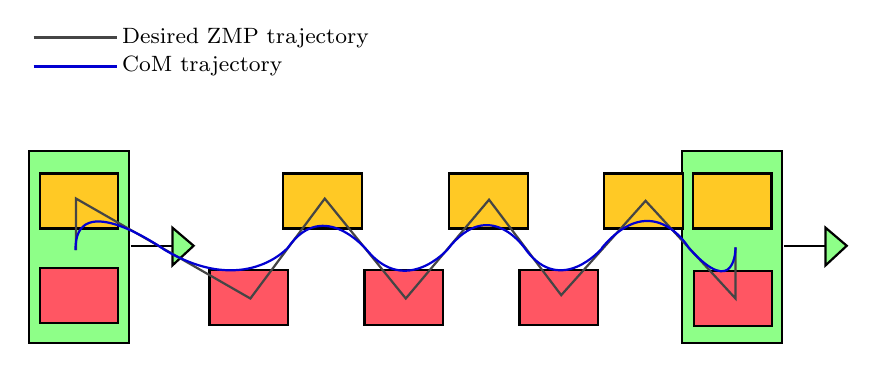
\begin{tikzpicture}[y=2.pt, x=2.pt,yscale=-1, inner sep=0pt, outer sep=0pt]
  %Start and end configurations
  \begin{scope}[cm={{0.0,1.0,-1.0,0.0,(360.33128,174.24827)}}]
    \path[draw=black,fill=c8eff88,miter limit=4.00,line width=0.800pt,rounded
      corners=0.0000cm] (47.0740,258.0597) rectangle (81.6792,276.2132);
    \path[draw=black,fill=c8eff88,line join=miter,line cap=butt,line width=0.800pt]
    (64.1273,257.7760) -- (64.1273,246.9973);
    \path[draw=black,fill=c8eff88,line join=miter,line cap=butt,line width=0.800pt]
    (64.1273,246.4300) -- (67.6730,250.2593) -- (60.8654,250.2593) -- cycle;
  \end{scope}
  \begin{scope}[cm={{0.0,1.0,-1.0,0.0,(478.33128,174.24827)}}]
    \path[draw=black,fill=c8eff88,miter limit=4.00,line width=0.800pt,rounded
      corners=0.0000cm] (47.0740,258.0597) rectangle (81.6792,276.2132);
    \path[draw=black,fill=c8eff88,line join=miter,line cap=butt,line width=0.800pt]
    (64.1273,257.7760) -- (64.1273,246.9973);
    \path[draw=black,fill=c8eff88,line join=miter,line cap=butt,line width=0.800pt]
    (64.1273,246.4300) -- (67.6730,250.2593) -- (60.8654,250.2593) -- cycle;
  \end{scope}
  %Footprints
    \path[cm={{0.0,1.0,-1.0,0.0,(0.0,0.0)}},draw=black,fill=cffc925,miter
      limit=4.00,line width=0.800pt,rounded corners=0.0000cm] (225.3161,-100.2912)
    rectangle (235.2439,-86.1087);
    \path[cm={{0.0,1.0,-1.0,0.0,(0.0,0.0)}},draw=black,fill=cffc925,miter
      limit=4.00,line width=0.800pt,rounded corners=0.0000cm] (225.3161,-144.2911)
    rectangle (235.2439,-130.1087);
    \path[cm={{0.0,1.0,-1.0,0.0,(0.0,0.0)}},draw=black,fill=cffc925,miter
      limit=4.00,line width=0.800pt,rounded corners=0.0000cm] (225.3161,-174.2911)
    rectangle (235.2439,-160.1087);
    \path[cm={{0.0,1.0,-1.0,0.0,(0.0,0.0)}},draw=black,fill=cffc925,miter
      limit=4.00,line width=0.800pt,rounded corners=0.0000cm] (225.3161,-202.2911)
    rectangle (235.2439,-188.1087);
    \path[cm={{0.0,1.0,-1.0,0.0,(0.0,0.0)}},draw=black,fill=cffc925,miter
      limit=4.00,line width=0.800pt,rounded corners=0.0000cm] (225.3161,-218.2911)
    rectangle (235.2439,-204.1087);
    \path[cm={{0.0,1.0,-1.0,0.0,(0.0,0.0)}},draw=black,fill=cff5663,miter
      limit=4.00,line width=0.800pt,rounded corners=0.0000cm] (242.4480,-100.2912)
    rectangle (252.3757,-86.1087);
    \path[cm={{0.0,1.0,-1.0,0.0,(0.0,0.0)}},draw=black,fill=cff5663,miter
      limit=4.00,line width=0.800pt,rounded corners=0.0000cm] (242.6932,-130.9444)
    rectangle (252.6209,-116.7619);
    \path[cm={{0.0,1.0,-1.0,0.0,(0.0,0.0)}},draw=black,fill=cff5663,miter
      limit=4.00,line width=0.800pt,rounded corners=0.0000cm] (242.6932,-158.9444)
    rectangle (252.6209,-144.7619);
    \path[cm={{0.0,1.0,-1.0,0.0,(0.0,0.0)}},draw=black,fill=cff5663,miter
      limit=4.00,line width=0.800pt,rounded corners=0.0000cm] (242.6932,-186.9444)
    rectangle (252.6209,-172.7619);
    \path[cm={{0.0,1.0,-1.0,0.0,(0.0,0.0)}},draw=black,fill=cff5663,miter
      limit=4.00,line width=0.800pt,rounded corners=0.0000cm] (242.8937,-218.4225)
    rectangle (252.8214,-204.2401);
  %ZMP trajectory
    \path[draw=c454545,line join=miter,line cap=butt,miter limit=4.00,line
      width=0.800pt] (92.6635,239.1801) -- (92.6635,229.8536) -- (124.1530,247.9049)
    -- (137.5913,229.8536) -- (152.2329,247.9049) -- (167.2757,230.0542) --
    (180.3127,247.3032) -- (195.5561,230.2548) -- (211.8023,247.9049) --
    (211.8023,238.6787);
  %Com trajectory
    \path[draw=c0200d1,line join=miter,line cap=butt,miter limit=4.00,line
      width=0.800pt] (92.5632,239.1801) .. controls (92.3626,227.5470) and
    (108.6088,239.0798) .. (108.6088,239.0798) .. controls (123.1502,247.7044) and
    (130.9724,238.6787) .. (130.9724,238.6787) .. controls (137.3907,229.5528) and
    (145.3132,239.2804) .. (145.3132,239.2804) .. controls (152.2329,247.5038) and
    (159.7543,239.0798) .. (159.7543,239.0798) .. controls (167.4762,229.0513) and
    (173.9948,239.1801) .. (173.9948,239.1801) .. controls (180.3127,247.5038) and
    (187.6336,238.8793) .. (187.6336,238.8793) -- (187.7338,238.6787) .. controls
    (196.9601,227.8479) and (203.3783,238.7790) .. (203.3783,238.7790) .. controls
    (211.9026,248.3061) and (211.8023,238.6787) .. (211.8023,238.6787);
  %legend
    \path[opacity=0,line join=miter,line cap=butt,line width=0.800pt]
    (85,200.7535) -- (100,200.7535)
    node[opacity=0,right] {\footnotesize Desired ZMP trajectory};
    \path[draw=c454545,line join=miter,line cap=butt,line width=0.800pt]
    (85,200.7535) -- (100,200.7535)
    node[right=2] {\footnotesize Desired ZMP trajectory};
    \path[draw=c0200d1,line join=miter,line cap=butt,line width=0.800pt]
    (85,206) -- (100,206)
    node[right=2] {\footnotesize CoM trajectory};

\end{tikzpicture}

  \caption{FIXME: Footprints, zmp, com, keep bounding box?}
  \label{fig:chap1-zmp}
\end{figure}

\subsection{Holonomic vs Nonholomic Walking Motion}
\label{subsec:chap1-holonomic}

Another important issue is the notion of holonomic motion: while
wheeled robots always remain tangent to their path, thus following a
nonholonomic constraint, legged robots can also move sideways, and
their motion can be described as holonomic. The path planning scheme
in \cite{yosh08} is designed to this end; a PRM algorithm first builds
a roadmap with Dubins curves \cite{dubi57}; but such curves impose a
nonholonomic constraint and narrow passages cannot be crossed. The
roadmap is therefore enriched with linear local paths. As a result
this planning scheme generates motion such that the robot remains
tangent to its path most of the time and uses sidestepping only in
narrow passages.

Furthermore, \cite{momb10} conducted a series of walking experiments
that allowed them to build a model of human walking trajectories; if a
human being walks long distances, his body tends to be tangential to
his path, while holonomic motion is used over smaller distances. This
is an attractive property for computed paths if a realistic motion is
to be achieved, and holonomic motion can as well be used to pass
through narrow spaces. These results suggest that a good combination
of both nonholonomic and holonomic motions can be used to achieve
realistic walking.

\subsection{Path Optimization}
\label{subsec:chap1-path-optimization}

Shortcut optimization, numerical methods (), A*, RRT* (or chapter 3?)

\subsection{Contribution: Regular Sampling Optimization}
\label{subsec:chap1-contribution}
The work of \cite{moul10} solves the walk planning problem
in a natural way, i.e. it uses numerical optimization to minimize the
robot walking along the path while following speed and obstacle
distance constraints. After having tried this approach, it was
empirically concluded that achieving successful numerical optimization
in any kind of environment is a difficult and computationally
expensive task; in fact, it requires computing a large set of
parameters to fully define the optimized path.

While using the same two-stage approach of \cite{yosh08}, a simpler
heuristic method that generates realistic time-optimal humanoid
trajectories is proposed. First the PRM algorithm and the Dubins local
paths are replaced with an RRT-Connect algorithm and linear local
paths. The path is then optimized by locally reorienting the robot
bounding box on a discrete set of configurations of the path. Priority
to nonholonomic motion is considered and holonomic motion is used only
to pass in narrow passages and to avoid nearby obstacles.

The following section presents this method and explains how it is
integrated in the motion planning scheme. Examples of different
scenarios, including a real one with the HRP-2 platform, are shown in
\autoref{sec:chap1-examples}.

\section{Optimization by Regular Sampling}
\label{sec:chap1-regular-sampling-optim}

\begin{figure}
  \centering
      {\includegraphics[width = 0.8\linewidth]
        {src/chap1-path-optimization/bb-plan-optim.pdf}}
      \caption{Top view: (a) RRT-Connect path for the bounding box
        passing between two chairs. (b) Optimized bounding box path by
        random optimization (RO). (c) Optimized bounding box after
        adding regular sampling optimization (RSO) .}
      \label{fig:chap1-bb-plan-optim}
\end{figure}

Assuming full knowledge of the environment, the RRT
algorithm produces a collision-free piecewise linear path $P_{RRT}$
for the robot bounding box (in offline mode), i.e. the path consists
of the concatenation of linear local paths $LP_{RRT}$.

Due to the probabilistic nature of RRT, $P_{RRT}$ may not be optimal
in terms of length, and a preliminary random shortcut optimization
(RO) can be run in order to shorten it (See
\autoref{fig:chap1-bb-plan-optim}). While the optimized path $P$ is
collision-free, the bounding box orientation is such that it could
lead to an unrealistic trajectory that is not time-optimal. For
instance, the humanoid robot could spend a long time walking sideways
or backwards over a long distance in an open space. An additional
optimization stage is introduced to address this issue in the next
section.

\subsection{Bounding Box Path Optimization}
Note that each configuration \config{} can be written as $q =
(\mathbf{X},~\theta)$, where $\mathbf{X} = (x,~y)$ describes the
bounding box position in the horizontal plane, and $\theta$ gives its
orientation.  The optimizer reorients the bounding box along $P$ by
changing $\theta$ while retaining the value of $\mathbf{X}$.

For this purpose, an A* search algorithm is executed; first $P$ is
regularly sampled. Using a discrete set of possible orientations for
each sample configuration and an adequate heuristic estimation
function, the bounding box orientation is then modified along $P$. An
optimized path $P_{opt}$ is created and leads to a realistic
time-optimal trajectory.

\subsubsection{Preliminary Notations}
After running RO on the piecewise linear path $P_{RRT}$, the
path $P$ is also piecewise linear, and its first and last
configurations are denoted by $q_s$ and $q_g$.

Let $d_{sample} \in \mathbb{R}_+^*$ be a sampling distance. Sampling
$P$ with a distance $d_{sample}$ means dividing each local path $LP_j$
of $P$ into smaller local paths of length $d_{sample}$; each new local
path end is a sample configuration. The $n^{th}$ sample configuration
of $P$ in its initial state can be obtained by indexing new local path
ends starting from $q_s$, and is denoted by $q_n^{init}$.

\begin{figure}
  \centering
      {\includegraphics[width = 0.75\linewidth]
        {src/chap1-path-optimization/A-star.pdf}}
      \caption{Each initial sample configuration can be rotated and be
        in one of four states. Starting from $q_s$, the A* search
        algorithm searches the graph $G$ that contains only valid
        nodes and arcs to produce an optimized path $P_{opt}$.}
      \label{fig:chap1-A-star}
\end{figure}

The possible orientation states need to be defined. We aim to make a
humanoid robot reach its goal as soon as possible. Since the robot is
faster while walking straight than side-stepping, we attempt to change
the orientation of each initial sample configuration $q_n^{init}$ such
that the bounding box is tangent to the local path and introduce a new
configuration denoted by $q_n^{front}$. To take into account the fact
that there may be obstacles that forbid a frontal orientation, we also
create $q_n^{lat_1}$ and $q_n^{lat_2}$ that are rotated by
$\frac{\pi}{2}$ and $-\frac{\pi}{2}$ relative to the path tangent, see
\autoref{fig:chap1-A-star}. One particular case is local path end
configurations: the mean direction of the two adjacent local paths is
considered to define frontal and lateral configurations. This is done
to ensure a smooth transition between two local paths.

A sample configuration whose orientation is unknown will be denoted by
$q_n^{state}$. It can have any orientation state of the set
$\{init,~front,~lat_1,~lat_2\}$ except for $q_s$ and $q_g$ which
remain in their initial state.  Ideally, the algorithm should be able
(as long as there are no obstacles) to put each sample configuration
in the frontal state, create a new path $P_{opt}$ and generate a
time-optimal trajectory for the robot.

An A* search is run to achieve this goal; the algorithm functions are
described in the following section.

\subsubsection{A* Function Definition}
\label{sec:chap1-A-star}
An A* search algorithm can find an optimal path in a graph
as long as a graph and an evaluation function are correctly
defined. Starting from $q_s$, A* expands in each iteration the
possible transitions from one sample to the next one in the graph and
evaluates with the evaluation function the cost of going through each
different state, see \autoref{fig:chap1-A-star}.

A graph $G$ is defined to be a set of nodes and arcs. A valid node
$q_n^{state_n}$ is defined to be a configuration with no collisions, and a valid arc
$q_n^{state_n}q_{n+1}^{state_{n+1}}$ is a collision-free local
path. The whole graph $G$ could be built before running A* by testing
all nodes and arcs and making sure they are collision-free. But
collision tests are slow, and A* uses a heuristic estimation function
to avoid going through all nodes. An empty graph $G$ is thus
initialized and nodes and arcs are built only when necessary. A
successor operator needs to be defined for this purpose.

\begin{figure}
  \centering
      {\includegraphics[width = 0.75\linewidth]
        {src/chap1-path-optimization/elliptic-constraint.pdf}}
      \caption{The rectangular bounding box speed vector $v$ is
        bounded inside the hashed area defined by the speed constraint
        $C$. The area is bounded by the union of two half-ellipsoids.}
      \label{fig:chap1-elliptic-constraint}
\end{figure}

\paragraph{The Successor operator $\Gamma(q_n^{state_n})$:}
Its value for any node $q_n^{state_n}$ is a set
$\{(q_{n+1}^{state_{n+1}},~c_{n,n+1})\}$, where
$q_{n+1}^{state_{n+1}}$ denotes a successor node, and $c_{n,n+1}$ is
the cost of going from $q_n^{state_n}$ to $q_{n+1}^{state_{n+1}}$. The
cost $c_{n,n+1}$ is defined to be the distance
$D(q_n^{state_n},~q_{n+1}^{state_{n+1}})$ between two nodes of $G$; it
computes the walk time from $q_n^{state_n}$ to
$q_{n+1}^{state_{n+1}}$. The speed constraint $C$ is defined as:
\begin{equation}
C = \left\{
\begin{array}{l l l}
  (\frac{v^{f}}{v_{max}^{f}})^2 +
  (\frac{v^{lat}}{v_{max}^{lat}})^2 - 1
  \quad \text{if } v^f >= 0 \\

  \\

  (\frac{v^{f}}{v_{min}^{f}})^2 +
  (\frac{v^{lat}}{v_{max}^{lat}})^2 - 1
  \quad \text{if } v^f < 0
\end{array} \right.
\end{equation}
where $v^{f}$ and $v^{lat}$ are respectively the frontal and lateral
speed, and $v_{min}^f$ $v_{max}^{f}$ and $v_{max}^{lat}$ their minimum
and maximum values (See
\autoref{fig:chap1-elliptic-constraint}). $D(q_n^{state_n},~q_{n+1}^{state_{n+1}})$
can be then computed by integrating this speed constraint along it.

Having expressed the successor operator, which allows the optimizer to
choose which node to expand at each iteration, the A* evaluation
function can be defined.

\paragraph{The Evaluation Function $\hat{f}(q_n^{state})$:}
It is the estimated cost of an optimal path going through
$q_n^{state}$ from $q_s$ to $q_g$ and can be written as:
\begin{equation}
  \hat{f}(q_n^{state}) = \hat{g}(q_n^{state}) + \hat{h}(q_n^{state})
\end{equation}
where $\hat{g}(q_n^{state})$ is the estimated cost of the optimal path
from $q_s$ to $q_n^{state}$ and $\hat{h}(q_n^{state})$ is a heuristic
function giving the estimated cost of the optimal path from
$q_n^{state}$ to $q_g$.

$\hat{h}(q_n^{state})$ must verify $\hat{h}(q_n^{state}) \leq
h(q_n^{state})$ to ensure that the algorithm is admissible, i.e. the
path from $q_s$ to $q_g$ is optimal. Since the robot is fastest while
walking straight forward in the absence of obstacles,
$\hat{h}(q_n^{state})$ is defined as:
\begin{equation}
  \begin{split}
  \hat{h}(q_n^{state}) &= D(q_n^{state},~q_{n+1}^{front}) \\
  &+ \sum_{k=1}^{N_{sample}-n-2} D(q_{n+k}^{front},~q_{n+k+1}^{front}) \\
  &+ D(q_{n+1}^{front},~q_g)
  \end{split}
\end{equation}
where $N_{sample}$ is the total number of initial sample
configurations in $P$ including $q_s$ and
$q_g$. $\hat{h}(q_n^{state})$ thus sums the cost of walking along $P$
while staying tangential to the path with the start and
end transition costs from $q_n^{state}$ and to $q_g$.

Now that the A* functions are fully defined, a search algorithm can be
run to compute an optimal path $P_{opt}$ by changing the orientation
of each sample node. An example is shown in
\autoref{fig:chap1-hash-direct-path}.

\begin{figure}
  \centering
      {\includegraphics[width = 0.75\linewidth]
        {src/chap1-path-optimization/hash-direct-path.pdf}}
      \caption{Local paths are regularly sampled (light grey) and each
        sample configuration is reoriented (dark) while considering
        obstacles $O_1$ and $O_2$.}
      \label{fig:chap1-hash-direct-path}
\end{figure}

\subsection{Motion Generation for a Humanoid Robot}

A collision-free path $P$ for the 3-DoF bounding box can be found
using RRT-Connect and RO. The regular sampling optimization (RSO),
which is the subject of this paper, is then applied on the path and
produces a path $P_{opt}$ that gives priority to nonholonomic motion.

Once the bounding box trajectory is computed, the robot has to walk
along it. A footstep sequence is thus generated along $P_{opt}$ by
geometric decomposition of the path, and the pattern generator cited
in \autoref{subsec:chap1-humanoid-walk-planning} then produces the robot
whole-body trajectory.

\section{Examples}
\label{sec:chap1-examples}

\begin{table}
\label{tab:chap1-computation-time}
\centering
\begin{tabular}{c|c|c|c|c|c|}
  \cline{2-6}
  & RRT-Connect & RO & RSO & Robot Trajectory & Total\\
  \hline
  \multicolumn{1}{|c|}{Chairs} & $3.97$ & $1.89$ & $2.14$ & $66.1$ & $74.1$\\
  \hline
  \multicolumn{1}{|c|}{Boxes} & $0.0917$ & $2.50$ & $0.238$ & $65.7$ & $68.6$\\
  \hline
  \multicolumn{1}{|c|}{Apartment} & $1.21$ & $2.43$ & $2.41$ & $223$ & $229$ \\
  \hline
\end{tabular}
\caption{Computational time (s) of each planning stage for the
  presented scenarios.}
\end{table}

\begin{table}
\label{tab:chap1-walk-time}
\centering
\begin{tabular}{c|c|c|}
  \cline{2-3}
  & RO & RO+RSO \\
  \hline
  \multicolumn{1}{|c|}{Chairs} & $40$ & $35$ \\
  \hline
  \multicolumn{1}{|c|}{Boxes} & $66$ & $57$ \\
  \hline
  \multicolumn{1}{|c|}{Apartment} & $200$ & $120$ \\
  \hline
\end{tabular}
\caption{Humanoid robot walk time (s) for the presented scenarios
  using RO alone and a RO-RSO combination.}
\end{table}

\begin{figure}
  \centering
      {\includegraphics[width = \linewidth]
        {src/chap1-path-optimization/chairs-hash-optim-perspective-hrp2.png}}
      \caption{Perspective view of the simulated HRP-2 trajectory on
        the final optimized path passing between two chairs.}
      \label{fig:chap1-chairs-hash-optim-perspective-hrp2}
\end{figure}

This section presents experimental results of the path
optimizer after it has been inserted in the previously described walk
planning scheme. Distance parameters $v_{max}^f$,
$v_{max}^{lat}$, $v_{min}^f$ are set to 0.5, 0.1, and 0.25
respectively. $d_{sample}$ is equal to $\frac{h}{6}$, where $h$
is the humanoid height.  Tests are performed on a 2.13 GHz Intel Core
2 Duo PC with 2 GB RAM.

Simulations of the humanoid robot HRP-2 are run in three scenarios.
The first one is a small environment where HRP-2 has to pass between
two chairs. The second environment is uncluttered with few obstacles
lying around, while the last one is a bigger apartment environment
where the robot has to move from one room to another while passing
through doors. The chairs scenario motion is also replayed on the real
robot HRP-2 (See \autoref{fig:chap1-hrp2-chairs}). Videos for all scenarios
can be viewed at \url{http://humanoid-walk-planning.blogspot.com/}

\begin{figure}
  \centering{
    \includegraphics[width = 0.75\linewidth]
                    {src/chap1-path-optimization/hrp2-chairs.png}}
  \caption{Humanoid Robot HRP-2 uses holonomic motion, or
    side-stepping, to pass between two chairs.}
  \label{fig:chap1-hrp2-chairs}
\end{figure}

\autoref{tab:chap1-computation-time} shows computation times for each stage
of the planning scheme: RRT-Connect, RO, RSO, and the whole-body robot
trajectory generation. In order to show the optimizer contribution,
robot walk times are also measured by creating a trajectory directly
after RO, and comparing it with a trajectory where the RSO was added.

\subsection{``Chairs'' Scenario}
\autoref{fig:chap1-bb-plan-optim} shows the bounding box RRT path
and the RO path for the chairs scenario. It is obvious that RO creates
a shorter path, but the bounding box starts rotating from the
beginning of the path even though the two chairs are still far. This
causes the robot trajectory to be unrealistic on one hand and, since
walking sideways takes a longer time than walking straight, to also
not be time-optimal.

\begin{figure}
  \centering
      {\includegraphics[width = \linewidth]
        {src/chap1-path-optimization/galton-hash-optim-perspective-hrp2.png}}
      \caption{Perspective view of HRP-2 optimized trajectory in the
        Galton board scenario.}
      \label{fig:chap1-galton-hash-optim-perspective-hrp2}
\end{figure}

However, after applying RSO, it is clear that the bounding box stays
oriented towards the front and rotates only when it reaches the
chairs. \autoref{fig:chap1-chairs-hash-optim-perspective-hrp2} and
\autoref{tab:chap1-computation-time} show that the walk time is shorter by 5
s and the final trajectory for HRP-2 is more realistic. Note that the
RSO takes 2,144 ms to be executed on the chairs path, which is less
than 3\% of the total computation time.

\subsection{``Galton'' Scenario}
An uncluttered environment is considered in this case, and
it can be seen that RRT-Connect and RSO computation times are very low
compared to other environments. This can be explained by the fact that
a tree connecting start and goal configurations is easier to find, and
that the frontal orientation state is valid for all considered samples
on the path (See \autoref{fig:chap1-galton-hash-optim-perspective-hrp2}).

\subsection{``Apartment'' Scenario}
The planning scheme is finally applied in the apartment
scenario. In \autoref{fig:chap1-apartment-hash-optim-perspective-hrp2}, it
is evident that HRP-2 walks facing forward through the doors. As with
previous scenarios, the trajectory is more realistic than a trajectory
where RSO is not used. The added computation time for RSO is 2,412 ms,
which is insignificant compared to the 228 s it takes for the whole
planning scheme.

Additionally, since the environment is significantly larger and more
constrained than the previous ones, the walk time difference is more
striking: \autoref{tab:chap1-computation-time} shows that it takes the robot
80 s less to cross the apartment when an RO-RSO combination is used.

\begin{figure}
  \centering
      {\includegraphics[width = \linewidth]
        {src/chap1-path-optimization/apartment-hash-optim-perspective-hrp2.png}}
      \caption{Perspective view of HRP-2 optimized trajectory in the
        apartment scenario.}
      \label{fig:chap1-apartment-hash-optim-perspective-hrp2}
\end{figure}

\section{Conclusion}
In this chapter, a novel simple optimization method is
presented for humanoid walk planning that relies on a decoupling
between trajectory and robot orientations. It uses an A* search that
takes as input a path for the robot bounding box, and produces a path
where a discrete set of configurations have been reoriented to generate
a realistic time-optimal walk trajectory. Results show that new
trajectories are more satisfactory while the added computation time is
insignificant compared to the whole planning time.

Of course, this approach can be used in other fields such as graphical
animation for digital actors to adapt the body orientation with respect
to the goal during locomotion. With a motion capture library
containing prerecorded nonholonomic and holonomic walk behaviors, it
is possible to lay this behavior on the actor trajectory and produce
realistic movements.

Discussion about drawback, possible improvements, transition to next
chapter.
